\documentclass[10pt, oneside]{amsart}
\usepackage[font={sf}]{caption}
\usepackage[]{graphics}
\usepackage{graphicx}
\usepackage{epstopdf}
\usepackage{hyperref}
\hypersetup{breaklinks=true, colorlinks=true, citecolor=blue}
\usepackage{natbib}
\usepackage{color}
\usepackage{soul}
\usepackage{rotating}
\usepackage{tabularx}
\usepackage{longtable}
\usepackage{lscape}
\usepackage{array}
\usepackage{multirow}
\usepackage{setspace}
\usepackage{textcomp}
\usepackage{dcolumn}
\setlength{\LTcapwidth}{6in}
\usepackage{dcolumn}
\usepackage[margin=1in]{geometry}
\usepackage{tocloft}
\usepackage{caption}

 \bibpunct{(}{)}{,}{a}{}{,}
 \doublespacing
 \raggedright
 \setlength{\parindent}{15pt} 


\begin{document}

\pagecolor{white}

\begin{center}
{ \Large \bf Figures }
\end{center}

\listoffigures

\begin{figure}[h]
	\begin{center}
		\includegraphics[width = 4.5 in]{Fig1_LAplots.pdf}
	\end{center}
	\caption[Local Adaptation]{The average amount of local adaptation that is reached in simulations that include inversions plotted as a function of migration rate and split between three panels representing weak, moderate and strong selection for a A) polygenic architecture and B) oligogenic architecture. The ribbon represents one standard deviation for the average local adaptation expected under the null which is the paired no-inversion control simulations. The difference between the average local adaptation reached in inversion simulations and the null paired no-inversion control simulation is shown for the C) polygenic architecture and D) oligogenic architecture. The percent of additive genetic variance (\%VA) found inside inverted regions is compared to the percent of the genome that is inverted. All averages are across five replicate simulations and all error bars represent one standard deviation. }
\end{figure}

\clearpage
\newpage

\begin{figure}[h]
	\begin{center}
		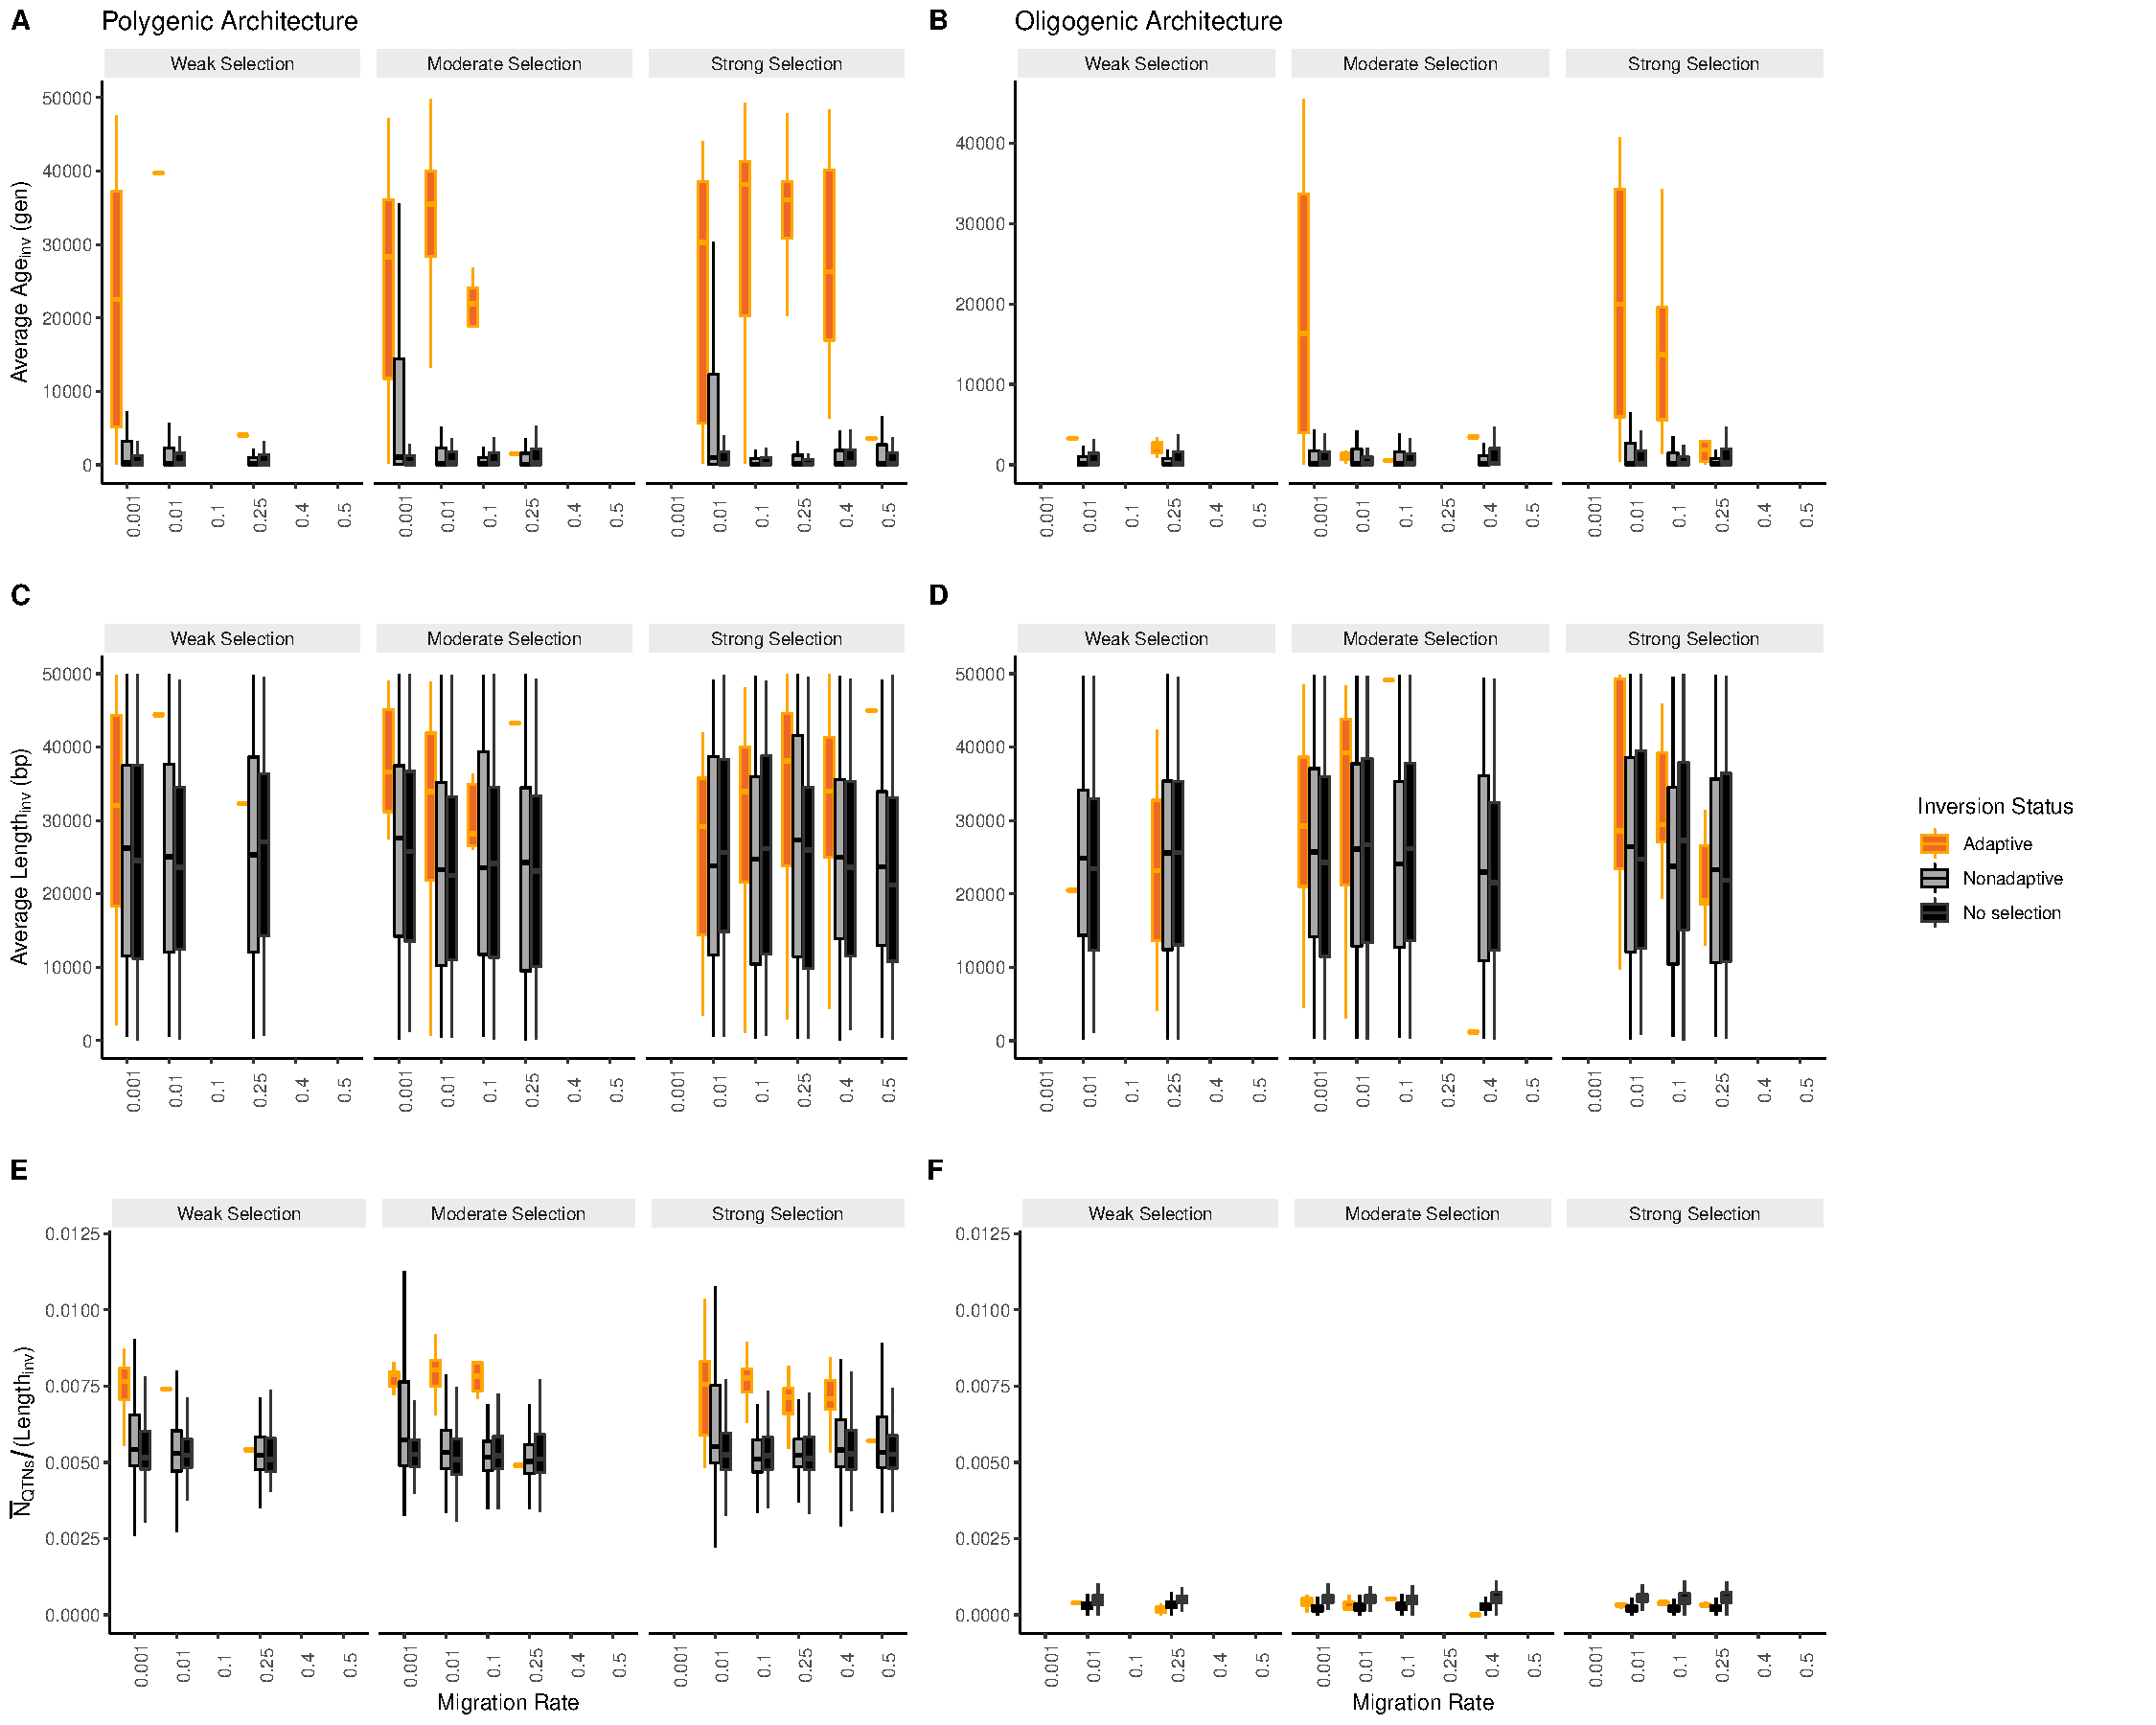
\includegraphics[width = 6.5 in]{Fig2_invChar_boxplot_noOutliers.pdf}
	\end{center}
	\caption[Inversion Characteristics]{The average of three inversion characteristics across five replicate simulations is plotted as a function of migration rate and split between three panels representing weak, moderate and strong selection for adaptive inversions in orange, nonadaptive inversions in light grey, and inversions from the no-selection control simulation in black. Inversion age in generations (gen) is plotted for a A) polygenic architecture and B) oligogenic architecture. Average inversion length in base pairs (bp) is plotted for a C) polygenic architecture and D) oligogenic architecture. Average number of inversion quantitative trait nucleotides (QTNs) scaled by the total length of the inversion plotted for a E) polygenic architecture and F) oligogenic architecture. Blank spaces represent those parameter combinations where no adaptive inversions evolved.}
\end{figure}

\clearpage
\newpage

\begin{figure}[h]
	\begin{center}
		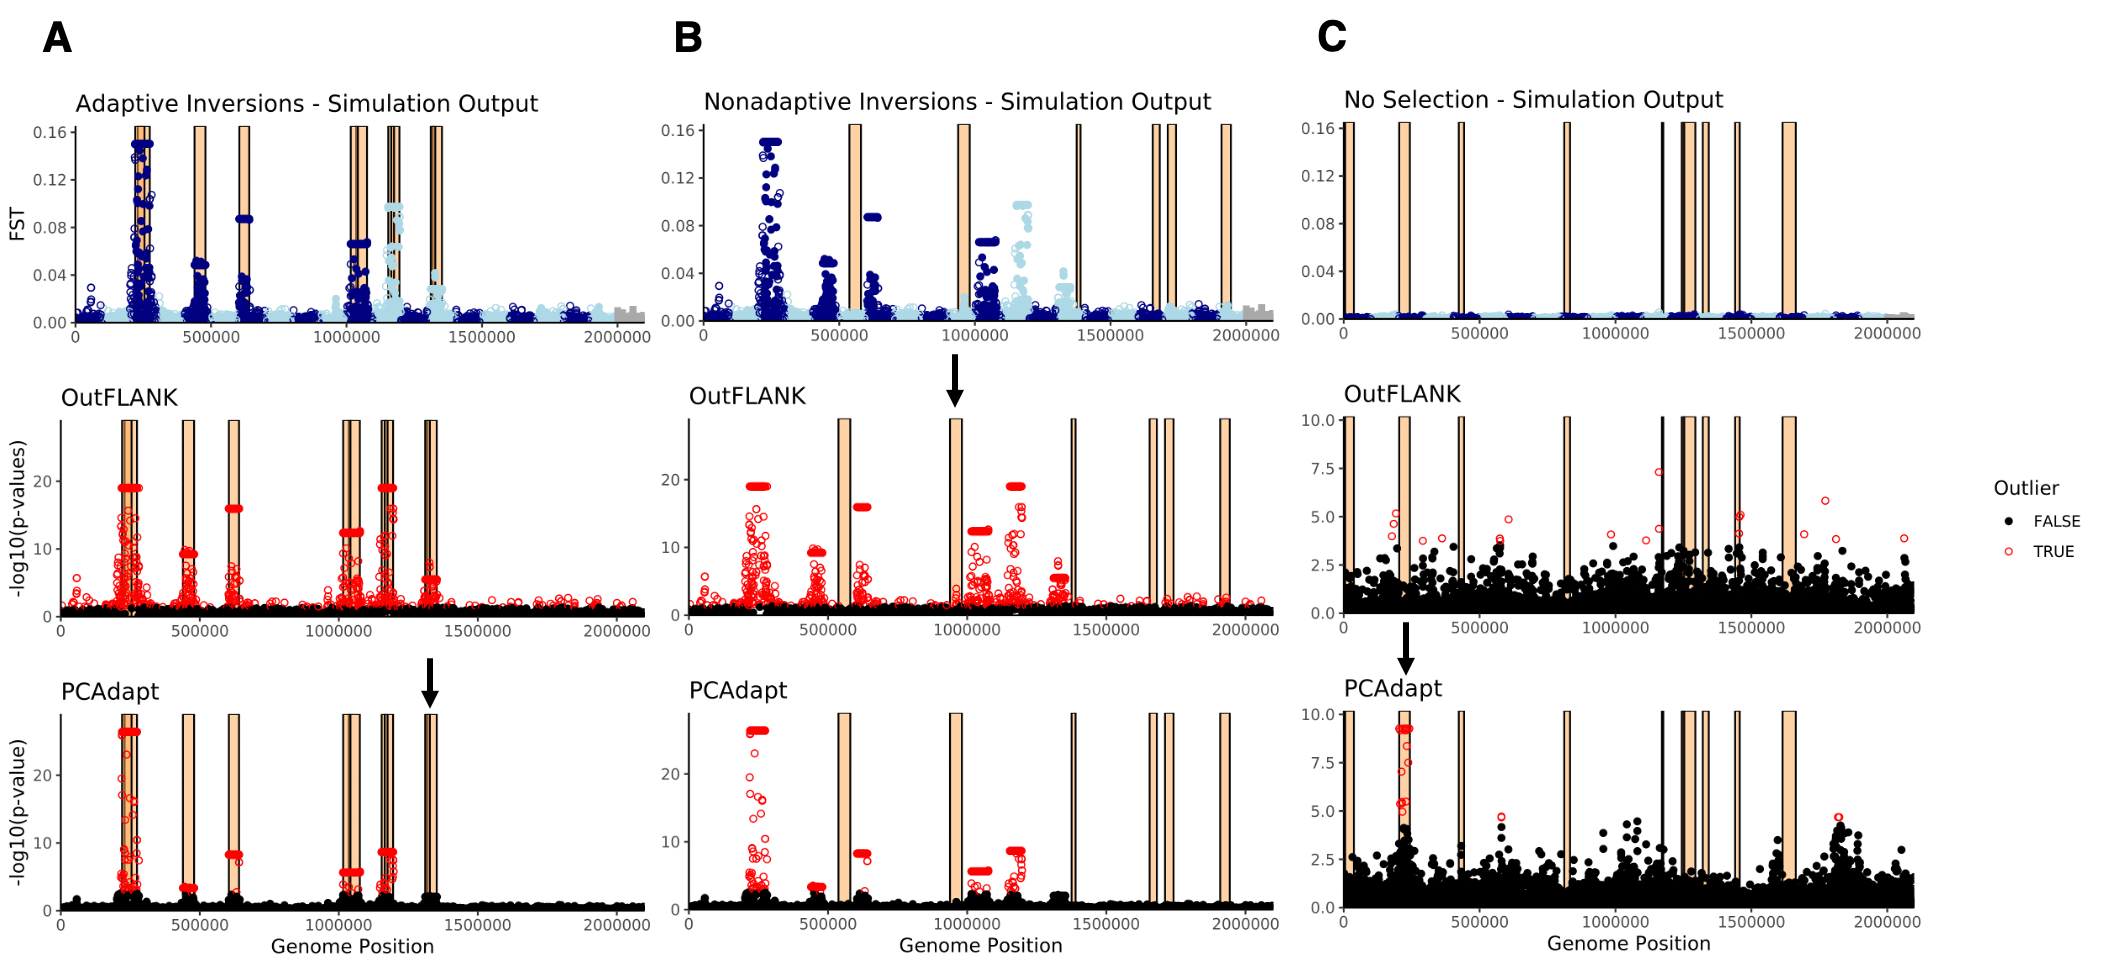
\includegraphics[width = 6.5 in]{Fig4_outlierExamples.pdf}
	\end{center}
	\caption[Outlier Examples]{Manhattan plots depicting either the FST of QTN loci (Top row across panels) or the empicial p-value for two different outlier detection methods, OutFLANK (middle row) and PCAdapt (bottom row), as a function of genomic position. Each point represents a QTN loci with alternating dark and light blue circles in the top panel representing each chromosome with loci under selection and light grey squares being the neutrally evolving chromosome. In the six outlier panels (middle and bottom rows), black filled in dots and red open circles represent nonoutlier and outlier loci, respectively. All gold bars represent inverted regions that are present in the simulation. Adaptive inversions are depicted in panel A with the black arrow identifying an inversion that was not identified as an outlier in PCAdapt. Panel B shows nonadaptive inversions with an arrow identifying an inversion that was called as an outlier in OutFLANK. Panel C shows inversions from the no-selection control simulation with an arrow identifying a nonadaptive inversion that was called as an outlier in PCAdapt.}
\end{figure}

\clearpage
\newpage


\begin{figure}[h]
	\begin{center}
		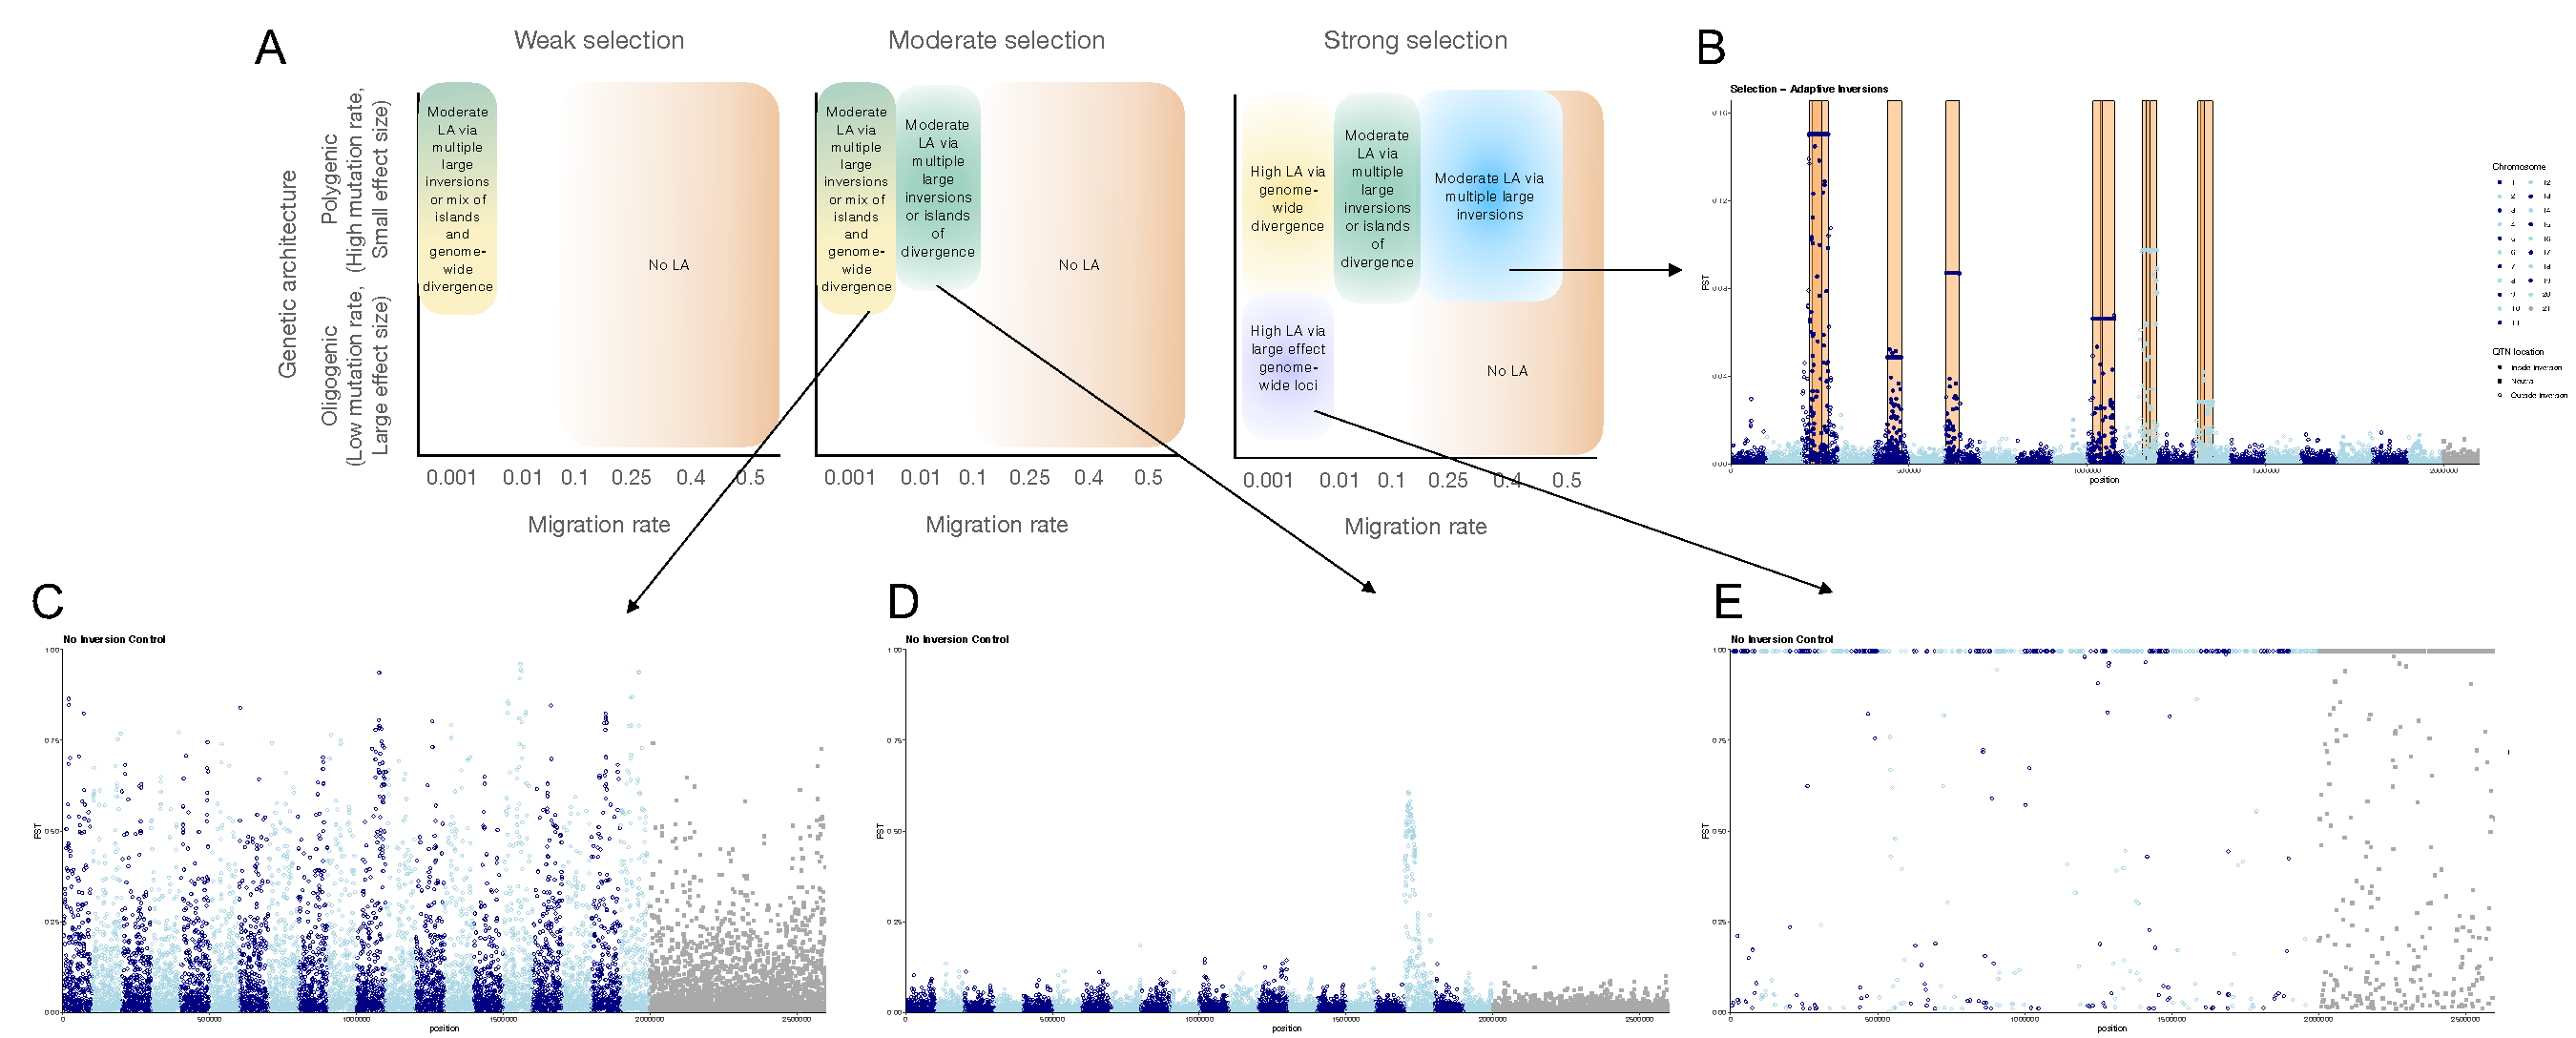
\includegraphics[width = 6.5 in]{Conceptual_with_manh.pdf}
	\end{center}
	\caption[ConceptualDiagram]{.}
\end{figure}


\end{document}